\chapter{Descubrimiento de procesos supervisado}
\label{chap:3}
En este capítulo, mostraremos en detalle como el enfoque utilizado en \cite{CarmonaC14} 
fue convertido en un proceso supervisado en \cite{LeonCB15}, y se vará cuales son las 
limitaciones de cada uno de los enfoques.

Para solventar estas limitaciones, se extenderá el enfoque de \cite{LeonCB15};
se propondrán diferentes métodos de mejora con el fin de
obtener, de manera automática y partiendo de los logs de un cierto sistema, 
un modelo que sea a la vez  adecuado, preciso, general y simple.

Se verá además, que la técnica utilizada es independiente del proceso de descubrimiento
y como puede ser utilizadp para simplificar los modelos obtenidos, por otras técnicas 
de descubrimiento de procesos.

\section{Algoritmo de descubrimiento}
\label{sec:3.algodisco}

Según lo visto en \autoref{sec:2.discovery discovery}, el descubrimiento de procesos
refiere al proceso mediante el cual, partiendo del log de un sistema, se busca
un modelo que lo represente.
Para este fin, existen diferentes metodologías \todo{citar metologías}.

En particular, en este trabajo, se basa en el algoritmo presentado en \cite{CarmonaC14}.
Este algoritmo, posee dos falencias. La primera, radica en el crecimiento exponencial de 
su complejidad con respecto al número de actividades en un log: se introduce una
estrategia del tipo \dquote{divide y vencerás}, utilizando los conceptos de muestreo -\textit{sampling}-
y proyección -\textit{projection}-.

    \todo[inline]{Resumir sampling}

    \todo[inline]{Resumir projection}


Las técnicas de muestreo y proyección, conforman una resolución satisfactoria al problema del
crecimiento exponencial de la complejidad que surge del enfoque monolítico, pero al mismo 
tiempo, la calidad de las métricas referentes a precisión y simplicidad suelen ser degradadas
considerablemente generando un modelo complejo y que admite demasiados comportamientos
por además de los provistos en el log inicial, i.e. \textit{underfitting}.

\begin{example}
Dado el siguiente log $\pmlog=\{ ac, abac, abab \}$, cuyo vector de Parikh es 
$\parikh{\pmlog}=\{ (0,0,0),(1,0,0), (1,0,1),\\(1,1,0), (2,1,0), (2,1,1),(2,2,0) \}$ (asuminedo el orden $(a,b,c)$).

Si se poryecta sobre las actividades $\{a,b\}$ y se utiliza una muestra con los puntos
$\{(1,0,1),(1,1,0),(2,1,1),(2,2,0)\}$, el conjunto de puntos proyectados es
$\{ (1,0), (1,1), (2,1), (2,2) \}$. 
Así, utilizando las técnicas en \cite{CarmonaC14}, se obtendá un modelo con
representado por la inecuación \mbox{$a \ge b$}.

Es claro que esto representa una subestimación del modelo ideal (si se consideran
todos los puntos del log), el cual se representa mediante la inecuación $a \ge b + c$.
\end{example}

La segunda limitación es que el algoritmo utilizado para computar el poliedro que contiene al 
conjunto de puntos en el conjunto de vectores de Parikh computa el \emph{mínimo} poliedro convexo 
o MCM por sus siglas en inglés (Minimum Convex Hull). Aunque en primer instancia puede parecer algo
positivo, computar la MCM implica generar restricciones innecesarias que generan luego un modelo
complicado del sistema. Exite en \cite{CarmonaC14} un post procesamiento de simplificación, pero este es
realizado de manera heurística y manuel, seleccionando un subconjunto de las restricciones que conforman la
$H$-representación del poliedro computado. Solo se utilizan las restricciones con coeficientes \dquote{simples}, 
eliminando el resto del modelo. 
Esta elección esta basada en la presunción de que, en la vida real, los procesos son definidos de manera
que sean \textit{simples} y más especialmente en el campo de la gestión de procesos de negocio. Esta presunción,
aunque no es necesariamente desacertada, puede que generalice demasiado el modelo, convirtiéndolo en un modelo
impreciso.

En el enfoque presentado, se utiliza la información negativa para poder detectar de manera automática
de las restricciones que se deberán eliminar es controlada mediante el uso de la información
negativa de manera de evitar una generalización muy grande. Un semiespacio será eliminado del modelo solo si esta acción
no introduce ningún punto negativo al sistema, en caso contrario, el semiespacio se mantiene. De esta manera, se
continúa con la idea básica de simplificar los modelos pero se restringe para evitar una generalización que degrade por
completo el modelo.

\subsection{Etapas del procedimiento propuesto}
\label{sec:3.algodisco stages}

\begin{figure}[t]
    \begin{center}
%\scalebox{1}{\input{img/flow.pdf_t}}
    \scalebox{.6}{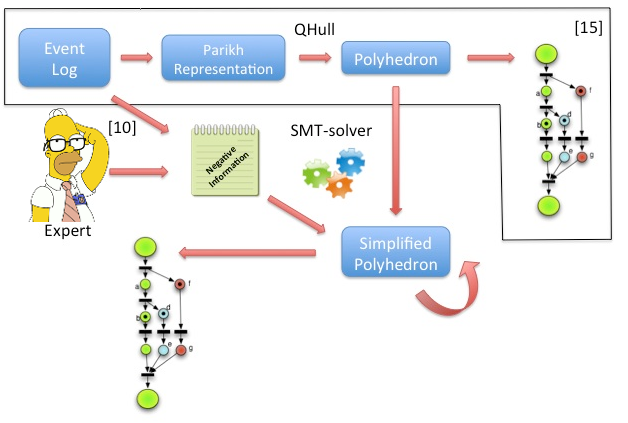
\includegraphics{img/approach_homero}}
    \caption{Procedimiento superviasdo propuesto (fuera del marco) en contraposición al enfoque
        en \cite{CarmonaC14} (dentro del marco).}
    \label{fig:flow}
    \end{center}
\end{figure}

El procedimiento propuesto para descubrimiento y simplificación de procesos se ilustra en \autoref{fig:flow}.

En la parte superior, dentro del marco negro, se representa el enfoque de \cite{CarmonaC14} en el cual se 
basa este trabajo. El detalle de como obtener el conjunto de vectores de Parikh a partír de un log,
de como un poliedro convexo que contenga dichos puntos y la relación existente entre dicho poliedo
y la red de Petri obtenida como modelo del sistema se puede ver en \autoref{chap:2}.

Por otro lado, la sección inferior de \autoref{fig:flow}, se ve como puede utilizarse infrormación negativa,
proveniente de diferentes medios, para simplificar el modelo obtenido a costo de aceptar mayor cantidad
de puntos. A continuación, se muestran los detalles de cada uno de los pasos propuestos en el presente trabajo.


\begin{algorithm}[h]
\caption{Descubrimiento de procesos supervisado}
  \begin{algorithmic}[1]
      \Require trazas positivas $\pmlog^+$ y trazas negativas $\pmlog_-$
      \Ensure una red de Petri $N$ donde $\forall \sigma \in \pmlog^+: \sigma \in L(N)$ y $\forall \sigma \in \pmlog_-: \sigma \not \in L(N)$
      \vspace{1mm}
      \Procedure{DISCOVER}{$\pmlog^+, \pmlog_-$}
      \State $pp, np \leftarrow \emptyset$ \label{algo:line1}
      \For{$\sigma_p \in \pmlog^+$}
        \For{$\sigma$ prefix of $\sigma_p$}
          \State add $\widehat\sigma$ to $pp$
       \EndFor
     \EndFor
      \For{$\sigma_n \in \pmlog_-$}
        \State add $\widehat\sigma_n$ to $np$
      \EndFor \label{algo:line2}
      \State $H$ = \textsc{ConvexHull}($pp$) \label{algo:lineqhull}
      \State $H_{smt}$ = \textsc{Shift\&Rotate}($H, np$)
      \State $H'$ = \textsc{Removal}($H_{smt}, np$)
      \State $N$ = \textsc{Hull2Net}($H'$)
      \State \Return N
      \EndProcedure
  \end{algorithmic}
  \label{algo}
\end{algorithm}

El \autoref{algo} detalla el enfoque utilizado paso a paso utiliando pseudocódigo. Un conjunto de trazas 
positivas y un conjunto de trazas negativas conformas la entrada (\dquote{log de eventos} e \dquote{información negativa} en \autoref{fig:flow}). 
En las líneas \ref{algo:line1}-\ref{algo:line2} se calculan todos los puntos positívos $pp$ para
cada prefijo de una traza positiva en $\pmlogp$ y los puntos negativos $np$ para las trazas en $\pmlogn$\footnotemark[1].
Luego, se calcula un poliédro que contenga el conjunto de puntos $pp$ mediante \textsc{ConvexHull} utilizando 
cualquier algoritmo que nos permita obtener la MCM para un conjunto de puntos, e.g. \qhulltool~\cite{Barber96}.

El poliedro que se obtiene es luego simplifcado mediante la función \textsc{Shift\&Rotate}, se uitlizan SMT-solvers,
en forma monolítica e iterativa. El resultado que se obtiene de un SMT-solver es una instancia de SMT, la cual
no necesariamente es la óptima (pueden existir múlples soluciones), por lo que se utiliza un proceso de refinamiento
iterativo para conseguir dicho óptimo.
La función \textsc{Removal} corresponde a la optimización del procedimiento manual presentado en \cite{CarmonaC14}.
En este punto, se considera la información negativa de $np$, eliminando únicamente aquellos hiperespacios
que no agreguen ningúno de los puntos de $np$ al modelo.

Por último, el conjunto de semiespacios es transformado en una red de Petri mediante \textsc{Hull2Net} utilizando
la dualidad que exuste entre los poliedros y las ecuaciones de marking de una red de Petri
presentada en \autoref{sec:2.discovery discovery}

Del hede de que \textsc{ConvexHull} puede depender de las técnicas de muestreo y proyección y del
hedho que que \textsc{Shift\&Rotate} está representado como una instancia de SMT la cual puede poseer múlples soluciones
y la devuelta depender de la implementación del solver, el algoritmo \autoref{algo} es no determinístico, i.e. dados
los mismos logs positivo y negativo de entrada se pueden obtener diferentes resultados.

\footnotetext[1]{ Nótese que en el caso de las trazas negativas, se utilizan únicamente los puntos correspondientes
    a cada traza completa y no a todos sus prefijos. Esto se debe a que para la mayor parte de las trazas negativas 
    el prefijo es compartido con alguna traza positiva por lo que no deben evitarse los prefijos.
}
    
\section{Generalización y simplificación}
\label{sec:3.gensimp}

En la \autoref{sec:2.discovery} se explica como partiendo de un conjunto de logs de un sistema, se pueden
obtener la MCH de del conjunto de vectores Parikh y luego, extrayendo la $H$-representación para
obtener un una red de Petri que modele dicho sistema; estos pasos corresponden a las líneas \ref{algo:line1}-\ref{algo:lineqhull} 
de \autoref{algo}. Sin embargo, la estructura de esta red suele ser muy compleja. Esto se debe a que no se está
buscando un poliedro arbitrario que contenga los puntos, sino que se calcula la MCM. La restricción de minimalidad
impuesta provoca restricciones irreales lo que genera modelos demasiado complejos, alejados del proceso existente lo que
implica que pierda el valor real. Por este motivo, luego de obtener el modelo, se realiza un post procesamiento para simplificar
el mismo.

Para simplificar un modelo, puede utilizarse información experta para detectar aquellas situaciones donde el modelo 
presentado es por demás restrictivo y puede relajarse. Al utilizar algoritmos de descubrimiento basados en un dominio
numérico abastracto, la simplificación consiste en remover de manera manual algunos de los semiespacios que definen
el poliedro de la $H$-representación. Debido a que cada semiespacio define un place en la red, al eliminarlos, se 
reduce el numero de places en la red y, por lo tanto, se obtiene un modelo más simple.

La propuesta de este trabajo es la de \dquote{desplazar} -\textit{shift}- y \dquote{rotar} -\textit{rotate}- el poliedro obtenido 
para obtener restricciones más simples, preservando, en la medida de lo posible, el comportamiento
original

Luego de estas simplificaciones, la red de Petri relacionada al poliedro acepta
una cantidad de trazas mayor, generalizando el comportamiento subyacente. Este procedimiento
de generalización se realiza de manera automática, verificando que no se introducen comportamientos
prohibidos.

\begin{example} 
    \label{ex:polyhedra}
    En \autoref{sfig:simp.1} se muestra un poliedro (el área gris claro) cuya $H$-representación viene
    dada por los semiespacios $\{p_0,p_1\}$ y algunas de las caminatas generadas por las trazas.
    Un poliedro más general, i.e. un poliedro cuyo $Z$-poliedro contiene más puntos, puede definirse
    mediante los semiespacioes $\{p_0,p_2\}$ (la unión de las areas gris clara y gris oscura). 
    
    Los puntos marcados mediante $\bullet$ no son solución de$\{p_0,p_1\}$ pero si lo son de $\{p_0,p_2\}$.
    La \autoref{sfig:simp.2} y la \autoref{sfig:simp.3} muestran las redes de Petri inferidas por cada uno 
    de los poliedros. 

    La secuencia de eventos $xxxyxxx$ (asumiendo la representación de los eventos siguiendo la usual de los 
    ejes cartesianos) es una traza de la red en \autoref{sfig:simp.3} pero no de la red en \autoref{sfig:simp.2}.
    Esto se ve representado en \autoref{sfig:simp.1} mediante el punto $(6,1)$, el cual es solución de $\{p_0,p_2\}$,
    pero no es solución de $\{p_0,p_1\}$.
\end{example}

El enfoque propuesto en \cite{LeonCB15} simplifica la $H$-representación de un poliedro modificando los semiescpacios
que lo componen. Para esto, se intenta reducir el valor absoluto de cada coeficiente de manera aislada; cada inecuación
simplificada debe incluír, al menos, las mismas soluciones que la original para evitar un modelo no adecuado. Sin embargo,
dado que el comportamiento del modelo no es definido por los semiespacios aislados sino por la conjunción de ellos,
es el modelo quien no debe perder soluciones y no un semiespacio particular.\todo{No me convence este ejemplo. No debería ser al revés? Un semiespacio \dquote{cree} que deja afuera a alguien pero en realidad no queda afuera? Esto habla de puntos que están afuera, por qué se controlaría eso?}\todo[inline]{A modo de ejemplo,
en la \autoref{fig:glob_encoding}, se tiene que el punto $(9,4)$ es una solución de \autoref{sfig:glob_encoding.1}.

s a solution on
the left for the half-space (call it $p$) bounding the grey polyhedron from below. If we try to simplify $p$ in isolation with the approach
from~\cite{LeonCB15}, the half-space $x = 8$ on the right could not be obtained since the solution $(9,4)$ of $p$ is lost. However
point $(9,4)$ is not part of the whole system (the one bounded by the conjunction of both half-spaces) and therefore this rotation (simplification) should
be allowed since the solution set on the right contains the solution set on the left.}

\begin{figure}[t]
  \centering
  \subbottom[\label{sfig:glob_encoding.1}]{%
    \scaledinput{0.40}{img/ineq1}}
  \hfill
  \subbottom[\label{sfig:glob_encoding.2}]{%
    \scaledinput{0.40}{img/ineq2}}
  \caption{Simplificación individual vs. simplificación matricial.}
  \label{fig:glob_encoding}
\end{figure}

La propuestra de esta tesina para mejorar el enfoque anterior, consiste en considerar
en el algoritmo de simplificación, la matriz de incidencia y el marking inicial como
una unidad no simplificar las inecuaciones una a una.
Dado un sistema de la forma,

\begin{center}
    $\begin{array}{rcccccccl}
        \alpha_{1,0} & + & \alpha_{1,1} \cdot x_1 & + & \dots & + & \alpha_{1,n} \cdot x_n & \ge & 0 \\
        \alpha_{2,0} & + & \alpha_{2,1} \cdot x_1 & + & \dots & + & \alpha_{2,n} \cdot x_n & \ge & 0 \\
            \vdots & & & & & & \vdots \\
        \alpha_{m,0} & + & \alpha_{m,1} \cdot x_1 & + & \dots & + & \alpha_{m,n} \cdot x_n & \ge & 0
    \end{array}$
\end{center}

se buscan nuevos coeficientes $\beta_{1,0},
\beta_{1,1}, \dots, \beta_{m,n}$ tal que:

\bequationl{enc1} \tag{NZ}
    \sum\limits_{i,j=1}^{m,n} \beta_{i,j} > 0 \text{ y } \sum\limits_{i=1}^{m} \beta_{i,0} > 0
\eequation

Para cada $0 \leq i \leq m$ y $1 \leq j \leq n$,

\bequationl{enc2} \tag{MIN}
    \rvert \beta_{i,j} \lvert\ \leq\ \rvert \alpha_{i,j} \lvert
\eequation

y para todo $x_j \ge 0$ con $1 \leq j \leq n$,

\bequationl{enc3}\tag{PC}
    \bigwedge\limits_{i=1}^m (\alpha_{i,0} + \sum\limits_{j=1}^n \alpha_{i,j} \cdot x_j )\ge 0 \ \Rightarrow\ \bigwedge\limits_{i=1}^m (\beta_{i,0} + \sum\limits_{j=1}^n \beta_{i,j} \cdot x_j) \ge 0
\eequation

Coloquialmente, \eqref{eq:enc1} especifica que al menos uno de los coeficientes debe ser no nulo,
para eliminar las soluciones triviales y que el marking inicial conste, cuanto menos, de un token.

El significado de \eqref{eq:enc2} por su parte, indica que la nueva matriz debe ser, al menos tan 
simple como la original.

Por último, cada solución del sistema inicial (como un todo) debe ser también una solución del nuevo
sistema para asegurar que mantenemos un modelo adecuado, de allí \eqref{eq:enc3}.


Para obtener la $H$-representación de un poliedro que implique una representación más simple y general de una red de Petri, 
las condiciones \eqref{eq:enc1}, \eqref{eq:enc2} y \eqref{eq:enc3} pueden ser codificadas utilizando 
teorías de satisfacibilidad módulo. 

Para la matriz de incidencia de \autoref{fig:simp.1}, por ejemplo, la codificación como SMT resulta

\todo{Esto no se puede ordenar más lindo? No me gusta...}
$$\begin{array}{c}
{(\beta_{1,1} + \beta_{1,2} + \beta_{2,1} + \beta_{2,2} > 0)} \land
{(\beta_{1,0} \geq 0)} \land
{(\beta_{2,0} \geq 0)} \land \\ \\
{(\lvert \beta_{1,1} \rvert \leq 2)} \land
{(\lvert \beta_{1,2} \rvert \leq 3)} \land
{(\lvert \beta_{2,1} \rvert \leq 1)} \land
{(\lvert \beta_{2,2} \rvert \leq 1)} \land \\ \\
{\forall \widehat\sigma(x), \widehat\sigma(y) : (6 - 2 \cdot \widehat\sigma(x) + 3 \cdot \widehat\sigma(y) \ge 0 \land 1 + \widehat\sigma(x) - \widehat\sigma(y) \ge 0)} \\ \\
\Rightarrow (\beta_{1,0} + \beta_{1,1} \cdot \widehat\sigma(x) + \beta_{1,2 }\cdot  \widehat\sigma(y) \ge 0 \land \beta_{2,0} + \beta_{2,1} \cdot \widehat\sigma(x) + \beta_{2,2} \cdot  \widehat\sigma(y) \ge 0)
\end{array}$$

para esta codificación, obtenemos, por ejemplo, la siguiente solución (mediante el uso de los SMT-Solvers)

$$\beta_{1,0}=6,\beta_{1,1}=-1,\beta_{1,2}=2, \beta_{2,0}=1,\beta_{2,1}=1,\beta_{2,2}=-1$$

correspondiente a la ecuacorres al marking de la red en \autoref{fig:simp.2}.

Se puede ver que el método propuesto no sacrifica lo adecuado de un modelo, ya que el $Z$-poliedro obtenido
contiene al original.

\begin{theorem}
    \label{theo:fit}
    Sea $\pmlog$ un log, $N$ un modelo adecuado de $\pmlog$ y $N'$ el modelo obtenido según el método propuesto,
    entonces $N'$ es adecuado para $\pmlog$.
\end{theorem}

\begin{proof}
    Sea $\mathcal{P} = \bigwedge\limits_{i=1}^m (\alpha_{i,0} + \sum\limits_{j=1}^n \alpha_{i,j} \cdot x_j )\ge 0$ y sean
    $\mathcal{P}' = \bigwedge\limits_{i=1}^m (\beta_{i,0} + \sum\limits_{j=1}^n \beta_{i,j} \cdot x_j )\ge 0$ los poliedros
    obtenidos de las ecuaciones de marking de $N$ y $N'$ su simplificación. Dado que $N$ es adecuado w.r.t. $\pmlog$, 
    todos los puntos correspondientes al conjunto de vectores Parikh de $\pmlog$ son solos puntos son solución de 
    $\mathcal{P}$. A partir de lo anterior y la constraint \eqref{eq:enc3}, todos los puntos también lo serán de $\mathcal{P}'$
    son ejecutables y por esto, se concluye que $N'$ también es adecuado para $\pmlog$.
\end{proof}


\subsection{Uso de información negativa}
\label{sec:3.gensimp negative}

El proceso de generalización y simplificación propuesto en \autoref{sec:3.gensimp} introduce puntos al modelo, 
los cuales generan nuevos comportamientos del sistema representado. Si se cuenta con un log negativo
(comportamientos prohibidos), puede agregarse esta información a la codificación para restringir la 
solución encontrada por el SMT-solver.

Para utilizar un log negativo, se procede a considerar la representación de las trazas (en este caso no se utilizan
los prefijos ya que algunos de ellos pueden coincidir con prefijos de alguna traza positiva) como vector Parihk.
Luego se consideran estos puntos como restricciones al aplicar la simplificación shift\&rotate; es decir, se debe 
verificar que las transformaciones realizadas al poliedro no conviertan a estos puntos en puntos válidos.

El enfoque presentado en \cite{LeonCB15}, considera las simplificaciones a realizar de manera aislada, limitando 
las simplificaciones realizadas a cada semiespacio a que no admita información negativa.
Esta restricción es muy estricta ya que un semiespacio puede contener un punto negativo siempre que exista otro semiespacio
que no lo admita. Si se considera \autoref{sfig:glob_encoding.2} como el modelo original y $(9,4)$ como un punto negativo,
el enfoque planteado en \cite{LeonCB15} no permitiría obtener la simplificación \autoref{sfig:glob_encoding.1} ya que una
de las inecuaciones lo acepta y sin embargo es claro que el punto prohibido no pertenece al poliedro.

\begin{figure}[t]
    \centering
    \begin{tikzpicture}

  \node[transition] (x) at (-.75,-1) {$x$};
  \node[transition] (y) at (.75,-1) {$y$};
  \node[tplace,label=above:$p_3$] (p1) at (0,0) {};
  \node[tplace,label=below:$p_0$] (p2) at (0,-2) {};
      
  \node[] (t) at (p1) {5};
  \node[] (t) at (p2) {1};
    
  \draw[style={->,>=triangle 45}] (p1) edge node[above left]{2} (x);
  \draw[style={->,>=triangle 45}] (x) to (p2);    
  \draw[style={->,>=triangle 45}] (p2) to (y);      
  \draw[style={->,>=triangle 45}] (y) edge node[above right]{2} (p1);

  \node[] (null) at (0,-3) {};
    
\end{tikzpicture}
    \caption{Petri net generated using negative information.}
    \label{fig:neg}
\end{figure}

Al igual que lo realizado al considerar las trazas positivas, el algoritmo de simplificación
puede ser optimizado si se consideran el conjunto comple de los semiespacios en lugar de uno
a la vez. 
Para evitar los comportamientos prohibidos, se utilizará la siguiente condición para cada 
uno de los puntos negativos $(k_1,\dots,k_n)$,

\bequationl{enc4} 
    \tag{NP}
    \begin{array}{rccccl}
        \bigvee\limits_{i=1}^m(\beta_{i,0} & + &\sum\limits_{j=1}^n \beta_{i,j} \cdot k_j) &< &0
    \end{array}
\eequation

Mediante esta representación, se fuerza a que, para cada punto negativo, al menos una de las inecuaciones no se satisfaga.

Si no se cuenta con información negativa, la restricción \eqref{eq:enc1} es necesaria para evitar 
la solución trivial, i.e. remover todos los semiespacios, esto no ocurre en el caso se conocen
comportamientos prohibidos; la solución trivial admitiría cualquier comportamiento negativo, por 
lo que podemos prescindir de \eqref{eq:enc1}.

\begin{example} 
    \label{ex:polyhedra_part2}
    Retomando el \autoref{ex:polyhedra}, si se desea generalizar y simplificar el modelo sin admitir el punto $(6,1)$,
    correspondiente al comportamiento $xxxyxxx$, utilizando la nueva representación, se debe agregar la restricción
    
    \bequation
        \begin{array}{lcr}
            (\beta_{1,0} + \beta_{1,1} \cdot 6 + \beta_{1,2} \cdot 1 < 0) &\lor& (\beta_{2,0} + \beta_{2,1} \cdot 6 + \beta_{2,2} \cdot 1 < 0)
        \end{array}
    \eequation

    la cual elimna $\beta_{1,0}=6,\beta_{1,1}=-1,\beta_{1,2}=2, \beta_{2,0}=1,\beta_{2,1}=1,\beta_{2,2}=-1$ 
    como una solución del sistema.

    Utilizar este algoritmo con información negativa, remplaza el primer semiespacio por 
    $5 -2 \cdot \widehat\sigma(x) +2 \cdot \widehat\sigma(y) \ge 0$ y mantiene el segundo.

    La red simplificada que se obtiene corresponde a la que se ve en \autoref{fig:neg}, donde
    se observa que no acepta $xxxyxxx$ como traza.
\end{example}

\subsection{Eliminación automática de semiespacios}
\label{sec:3.removal}

El ultimo aspecto de este nuevo aspecto consiste en la eliminación automática 
de los semiespacios, realizada mediante el procedimiento \textsc{Removal}.
Este procedimiento toma como argumento un poliedro y un conjunto de puntos
negativos e itera sobre los los semiespacios verificando si el poliedro
que se obtiene al eliminandolo acepta alguno de los puntos negativos.
Si este no es el caso, la restricción puede ser eliminada sin incorporar
ningún comportamiento prohibido al modelo del sistema. El procedimiento 
que realiza esto corresponde a \autoref{algo:rem}. $\textsc{SomeInside}(H \setminus h, np)$
retorna \textit{true} si eliminar $h$ tiene como consecuencia que algún punto en $np$
sea una solución de $H$.

\begin{algorithm}[h]
\caption{Eliminación automática de semiespacios}
    \begin{algorithmic}[1]
        \Procedure{Removal}{$H, np$}
            \For{$h \in semiespacios(H)$}
                \If{$\neg \textsc{SomeInside}(H \setminus h, np)$}
                    \State eliminar $h$ de $H$
                \EndIf
            \EndFor
            \State \Return $H$
        \EndProcedure
    \end{algorithmic}
    \label{algo:rem}
\end{algorithm}

El resultado de este procedimiento depende de la calidad de la información negativa:
un mal conjunto de trazas prohibidas puede permitir remover demasiados semiespacios,
deteriorando la precisión de la red de Petri final. Como puede verse en los experimentos,
las trazas que se obtienen en ~\cite{BrouckeWVB14} permiten remover semiespacios sin 
impactar en gran medida la calidad de las métricas de la red.

\subsection{Conceptos de complejidad}
\label{sec:3.complexity}

Existen diferentes conceptos de complejidad referidos a las redes de Petri \cite{Lassen08}\cite{Mendling2007},
la mayor parte se centran en la simpleza visual del modelo final. Sin embargo, estás métricas usualmente 
son definidas en una clase de redes de Petri más restrictiva, donde el principal objetivo radica en la 
representación de flujos de trabajo. Por su parte, las redes utilizadas en este trabajo resultan más generales
y permiten representar conceptos como recursos y costos. Por este motivo, se utiliza una definición más adecuada
de complejidad para medir la eficiencia buscada.

La idea principal radica en minimizar los coeficientes correspondientes a la matriz de incidencia de la red.
La complejidad de una cierta red resulta de la suma de los valores absolutos de los tokens iniciales, 
los tokens consumidos y los tokens producidos por cada transición.

Dada una re de Petri cuyo marking inicial sea $(\alpha_{1,0}, \dots, \alpha_{m,0})$ y su matriz de incidencia

\begin{equation*}
\left(\begin{array}{ccc} \alpha_{1,1} & \dots & \alpha_{1,n} \\  \vdots & & \vdots \\ \alpha_{m,1} & \dots & \alpha_{m,n}\end{array} \right)
\end{equation*}

su \textit{complejidad estructural} viene dada por 

\bequation
    \sum\limits_{i=1}^m (\lvert \alpha_{i,0} \rvert + \sum\limits_{j=1}^n \lvert \alpha_{i,j} \rvert).
\eequation

Utilizando esta definición, la complejidad de los poliedros \autoref{fig:simp.1} y \autoref{fig:simp.2} es 14 y 12 respectivamente.
Por lo tanto, la red correpondiente a \autoref{fig:simp.2} es considerada más simple.
La efectividad del método presentado se define como la reducción de la complejidad del nuevo poliedro.

\begin{example}
    \autoref{fig:mot} muestra el resultado de aplicar el método presentado; la red \autoref{2fig:mot1} posee
    complejidad $c_1 = (6 + 2 + 3) + (1 + 1 + 1) + (2 + 1) + (1+1+1) + (3+1) + 1 = 25$ mientras que 
    la red \autoref{2fig:mot2}, obtenida luedo de aplicar el algoritmo presentado, posee complejidad 
    $c_2 = (2+1+1) + (1+1+1) + (2+1) + (1+1) + (3+1) + 1 = 17$. En este ejemplo, la eficiencia del
    procedimiento es $100 - 100 \times (c_2 / c_1) = 32\%$.
\end{example}


Es importante destacar que existen casos donde las nociones de complejidad coinciden en el sentido de indicar
qué red es más simple, debido a que, remover un semiespacio, es equivalente a simplificar todos sus coeficientes
hasta cero. Sin embargo, este no es siempre el caso. Siguiendo la definición aquí propuesta, una red que contenga
dos places y coeficientes pequeños (en valor absoluto) es más simple que una red que contenga un único place con 
coeficientes altos lo cual contradice las métricas que se ocupan en la simplicidad visual (e.g. contar la cantidad
de places de una red).

\subsection{Simplificación de modelos arbitrarios}
\label{sec:3.simplification}

Es importente observar que las técnicas presentadas en la sección anterior es independiente al algoritmo de 
descubrimiento presentado en \cite{CarmonaC14} y pueden ser aplicadas sobre cualqueir
red de Petri que satisfaga los supuestos, i.e. una red de Petri pura, sin transiciones silenciosas y sin
dos transiciones representando una misma acción. 

En \autoref{sec:3.discovery}, se explica la correspondencia entre un poliedro y una de de Petri mediante
la $H$-representación de la ecuacuión de marking de $\mathcal{P}$. Esta relación es utilizada en \cite{CarmonaC14}
para computar $N$ a partir de $\mathcal{P}$. Para utilizar el algorimos de simplificación anterior, se utiliza
esta correspondencia en la otra dirección, computando $\mathcal{P}$ a partir de $N$. Para esto, se toma la matriz
de adyacencia de $N$ como el marking iniciat y se utiliza la $H$-representación del poliedro correspondiente 
a $N$. De esta manera, se puede obtener una red de Petri mediante una técnica de descubrimiento arbitrario
y sobre ella aplicar la codificación como SMT como un procesamienti posterior para simplificar el modelo.

\section{Resumen del capítulo}
\label{sec:3.resumen}

En este capítulo se presentó la teoría sobre los métodos utilizados para obtener una red de Petri
a partir de un log de manera automática y como este método puede mejorarse mediante el uso de información
negativa y se especificó el concepto de complejidad utilizado para obtener las métricas de una red de
Petri dada.

Además se definió lo que consiste en el mayor aporte del presente trabajo, el  algoritmo de
generalización y simplificación utilizado SMT-solvers e información negativa.
Luego de esto, se procede a un proceso de eliminación automática controlada mediante el cual se intenta 
generar un modelo que tenga la capacidad de capturar comportamientos no observados en el log.

Todo el proceso descripto ha sido implementado de manera integral como parte de este trabajo
y los detalles sobre dicha implementación serán discutidos en el siguiente capítulo.
